\documentclass{report}
% Include all project wide packages here.
\usepackage{fullpage}
\usepackage[style=ieee]{biblatex}
\usepackage[dutch]{babel}

\renewcommand{\familydefault}{\sfdefault}

\setmainfont[Ligatures=TeX]{Myriad Pro}
\setmathfont{Asana Math}
\setmonofont{Lucida Console}

\usepackage{titlesec, blindtext, color}
\definecolor{gray75}{gray}{0.75}
\newcommand{\hsp}{\hspace{20pt}}
\titleformat{\chapter}[hang]{\Huge\bfseries}{\thechapter\hsp\textcolor{gray75}{|}\hsp}{0pt}{\Huge\bfseries}
\renewcommand{\familydefault}{\sfdefault}
\renewcommand{\arraystretch}{1.2}
\setlength\parindent{0pt}

%For code listings
\definecolor{black}{rgb}{0,0,0}
\definecolor{browntags}{rgb}{0.65,0.1,0.1}
\definecolor{bluestrings}{rgb}{0,0,1}
\definecolor{graycomments}{rgb}{0.4,0.4,0.4}
\definecolor{redkeywords}{rgb}{1,0,0}
\definecolor{bluekeywords}{rgb}{0.13,0.13,0.8}
\definecolor{greencomments}{rgb}{0,0.5,0}
\definecolor{redstrings}{rgb}{0.9,0,0}
\definecolor{purpleidentifiers}{rgb}{0.01,0,0.01}


\lstdefinestyle{csharp}{
language=[Sharp]C,
showspaces=false,
showtabs=false,
breaklines=true,
showstringspaces=false,
breakatwhitespace=true,
escapeinside={(*@}{@*)},
columns=fullflexible,
commentstyle=\color{greencomments},
keywordstyle=\color{bluekeywords}\bfseries,
stringstyle=\color{redstrings},
identifierstyle=\color{purpleidentifiers},
basicstyle=\ttfamily\small}

\lstdefinestyle{c}{
language=C,
showspaces=false,
showtabs=false,
breaklines=true,
showstringspaces=false,
breakatwhitespace=true,
escapeinside={(*@}{@*)},
columns=fullflexible,
commentstyle=\color{greencomments},
keywordstyle=\color{bluekeywords}\bfseries,
stringstyle=\color{bluestrings},
identifierstyle=\color{purpleidentifiers}
}

\lstdefinestyle{vhdl}{
language=VHDL,
showspaces=false,
showtabs=false,
breaklines=true,
showstringspaces=false,
breakatwhitespace=true,
escapeinside={(*@}{@*)},
columns=fullflexible,
commentstyle=\color{greencomments},
keywordstyle=\color{bluekeywords}\bfseries,
stringstyle=\color{redstrings},
identifierstyle=\color{purpleidentifiers}
}

\lstdefinestyle{xaml}{
language=XML,
showspaces=false,
showtabs=false,
breaklines=true,
showstringspaces=false,
breakatwhitespace=true,
escapeinside={(*@}{@*)},
columns=fullflexible,
commentstyle=\color{greencomments},
keywordstyle=\color{redkeywords},
stringstyle=\color{bluestrings},
tagstyle=\color{browntags},
morestring=[b]",
  morecomment=[s]{<?}{?>},
  morekeywords={xmlns,version,typex:AsyncRecords,x:Arguments,x:Boolean,x:Byte,x:Char,x:Class,x:ClassAttributes,x:ClassModifier,x:Code,x:ConnectionId,x:Decimal,x:Double,x:FactoryMethod,x:FieldModifier,x:Int16,x:Int32,x:Int64,x:Key,x:Members,x:Name,x:Object,x:Property,x:Shared,x:Single,x:String,x:Subclass,x:SynchronousMode,x:TimeSpan,x:TypeArguments,x:Uid,x:Uri,x:XData,Grid.Column,Grid.ColumnSpan,Click,ClipToBounds,Content,DropDownOpened,FontSize,Foreground,Header,Height,HorizontalAlignment,HorizontalContentAlignment,IsCancel,IsDefault,IsEnabled,IsSelected,Margin,MinHeight,MinWidth,Padding,SnapsToDevicePixels,Target,TextWrapping,Title,VerticalAlignment,VerticalContentAlignment,Width,WindowStartupLocation,Binding,Mode,OneWay,xmlns:x}
}

%defaults
\lstset{
basicstyle=\ttfamily\small,
extendedchars=false,
numbers=left,
numberstyle=\ttfamily\tiny,
stepnumber=1,
tabsize=4,
numbersep=5pt
}

\title{Meetrapport: Opamps - Werking \& Afleiding}
\author{Robin Hes\\\&\\Erwin R. de Haan}

\begin{document}
\chapter{Werking \& Afleiding}

\section{Theorie}
Een relaxatie-oscillator maakt het, zoals al gezegd, mogelijk om een analoog signaal op een manier te coderen die bruikbaar is voor digitale systemen. Dit betekent dat een bepaald spanningsniveau moet worden omgezet naar een reeks ``enen en nullen'' of equivalenten daarvan die door het digitale systeem zijn te onderscheiden als twee verschillende waarden. Een relaxatie-oscillator bereikt dit doel door het analoge signaal om te zetten naar een bloksignaal met een periode die afhankelijk is van de waarde van het ingangssignaal.

\begin{figure}[H]
	\centering
	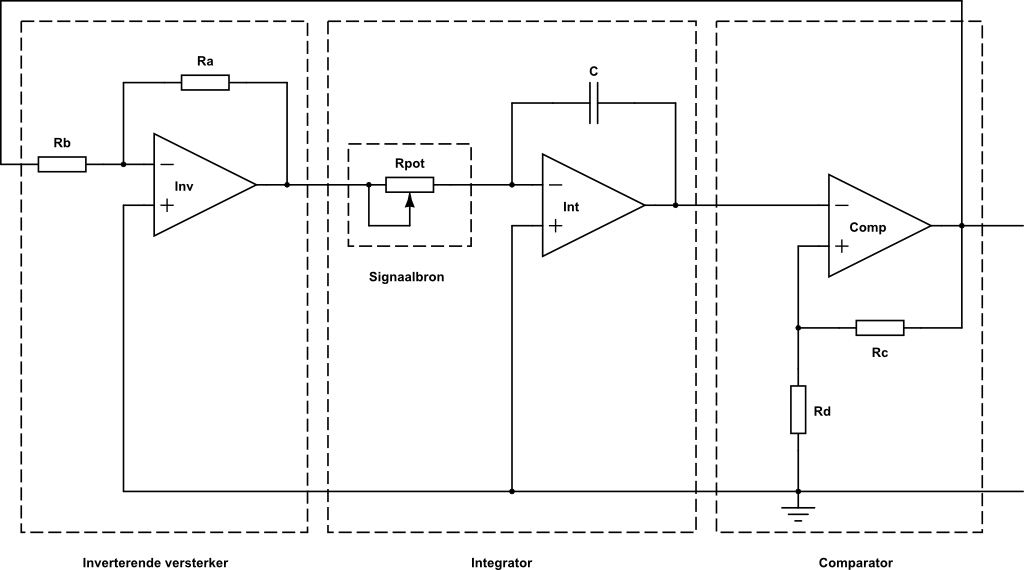
\includegraphics[width=0.8\textwidth]{relaxatie-oscillator.png}
	\caption{De relaxatie-oscillator}
	\label{fig:rel-os}
\end{figure}

Zoals te zien in figuur \ref{fig:rel-os} bestaat de relaxatie-oscillator uit drie afzonderlijke onderdelen: een integrator, een comparator en een inverterende versterker, allen gebaseerd op een op-amp met terugkoppelcircuit. We zullen hieronder per onderdeel een beschrijving geven van de functie in het geheel.

\subsection{Integrator}

De eerste stap in het digitaliseren van het ingangssignaal is om het signaal te integreren. Het signaal is op een punt in de tijd constant, waardoor integratie een lineaire functie oplevert. Als we een blokgolf zouden invoeren - dit is namelijk het uiteindelijke uitgangssignaal, wat weer teruggevoerd wordt in de ingang (zie figuur \ref{fig:rel-os} -  betekent dit dat de integrator een driehoekige functie oplevert, bij de overgang van hoog naar laag levert integratie een dalende lineaire functie op, bij de overgang van laag naar hoog is deze stijgend.\\

\begin{wrapfigure}{r}{0.5\textwidth}
	\centering
	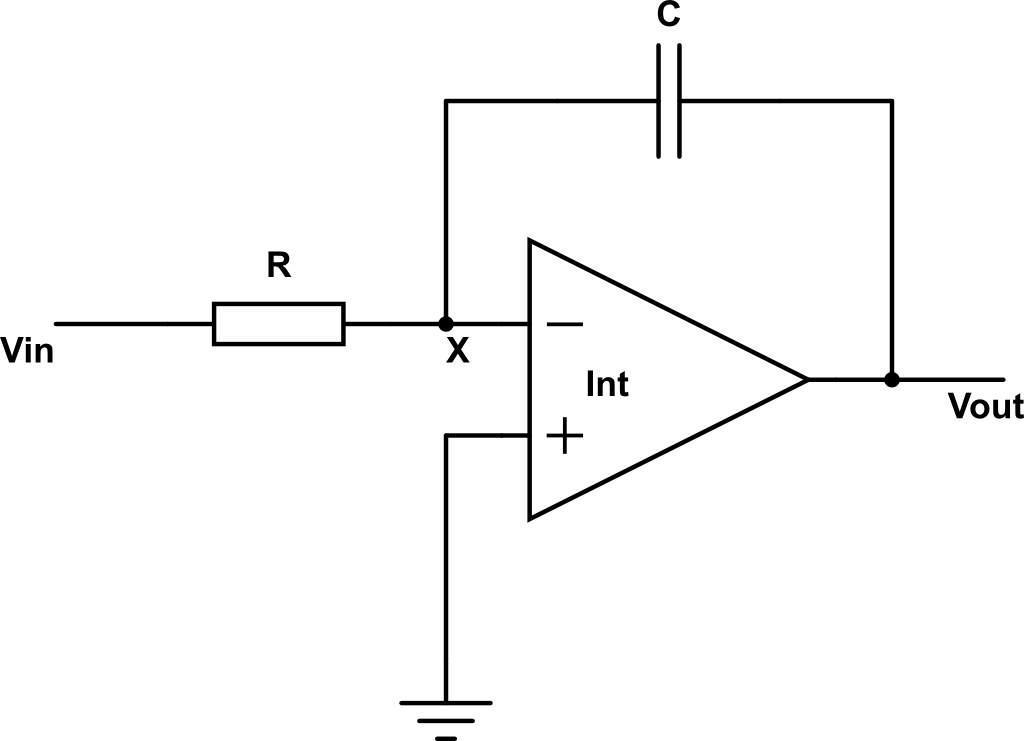
\includegraphics[width=0.4\textwidth]{integrator.png}
	\caption{De relaxatie-oscillator}
	\label{fig:int}
\end{wrapfigure}

De integrator, zoals weergegeven in figuur \ref{fig:int}, zou gezien kunnen worden als een inverterende spanningsversterker met een capaciteit in het terugkoppelcircuit, in plaats van een weerstand. Om de uitgangsspanning te berekenen als functie van de ingangsspanning gebruiken we de eigenschap dat de stroom door een condensator evenredig is met de afgeleide naar de spanning over de tijd:

$$I_{C} = C\frac{dv}{dt}$$

\noindent
Volgens Kirchhoff geldt ook:

$$I_{C} = -\frac{V_{in}}{R}$$

\noindent
En dus geldt ook:

$$C\frac{dv}{dt} = -\frac{V_{in}}{R}$$

\noindent
Na integreren vinden we hieruit een uitdrukking:

\begin{equation}
	V_{out} = -\left\lbrack\int \frac{V_{in}}{RC} \mathrm{d}t + V_{0}\right\rbrack = -\frac{V_{in}}{RC} t - V_{0}
	\label{eq:int}
\end{equation}

\noindent
Het door de integrator geleverde signaal voeren we vervolgens in de comparator, het volgende onderdeel.

\subsection{Comparator}

De integrator levert ons een driehoekig signaal, waar wij een blokgolf nodig hebben. Er is dus nog een bewerking nodig voordat het signaal gebruikt kan worden met een FPGA. Het driehoekige signaal moet worden omgezet in een blokgolf en de comparator is het component dat deze taak voor zijn rekening neemt. De blokgolf die door deze comparator wordt gegenereerd dient vervolgens niet alleen als digitaal signaal voor de FPGA, maar ook als ingangsspanning voor de relaxatie-oscillator zelf, waardoor deze continu oscilleert, vandaar de naam.

\begin{figure}[H]
	\centering
	\begin{subfigure}{0.5\textwidth}
		\centering
		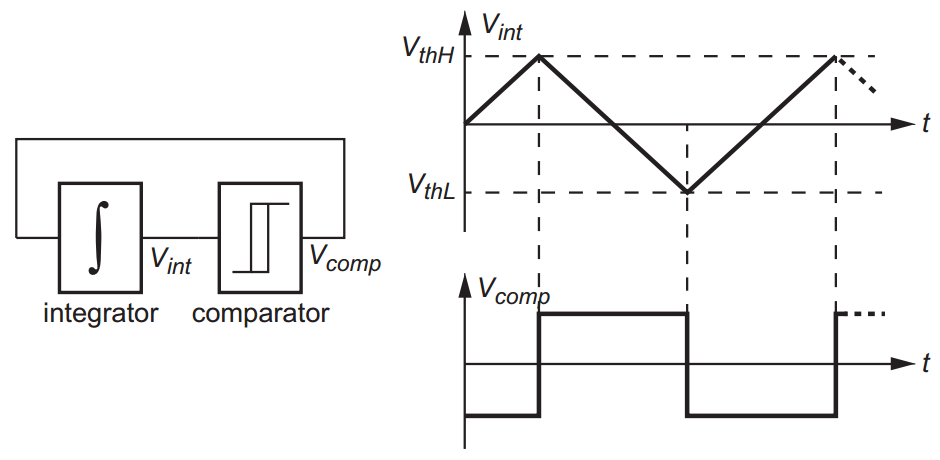
\includegraphics[width=\textwidth]{comparator-werking.png}
		\caption{De schematische werking van een comparator met hysterese. Naar: \cite{epo2-opamps}}
		\label{fig:comp-werk}
	\end{subfigure}
	\begin{subfigure}{0.4\textwidth}
		\centering
		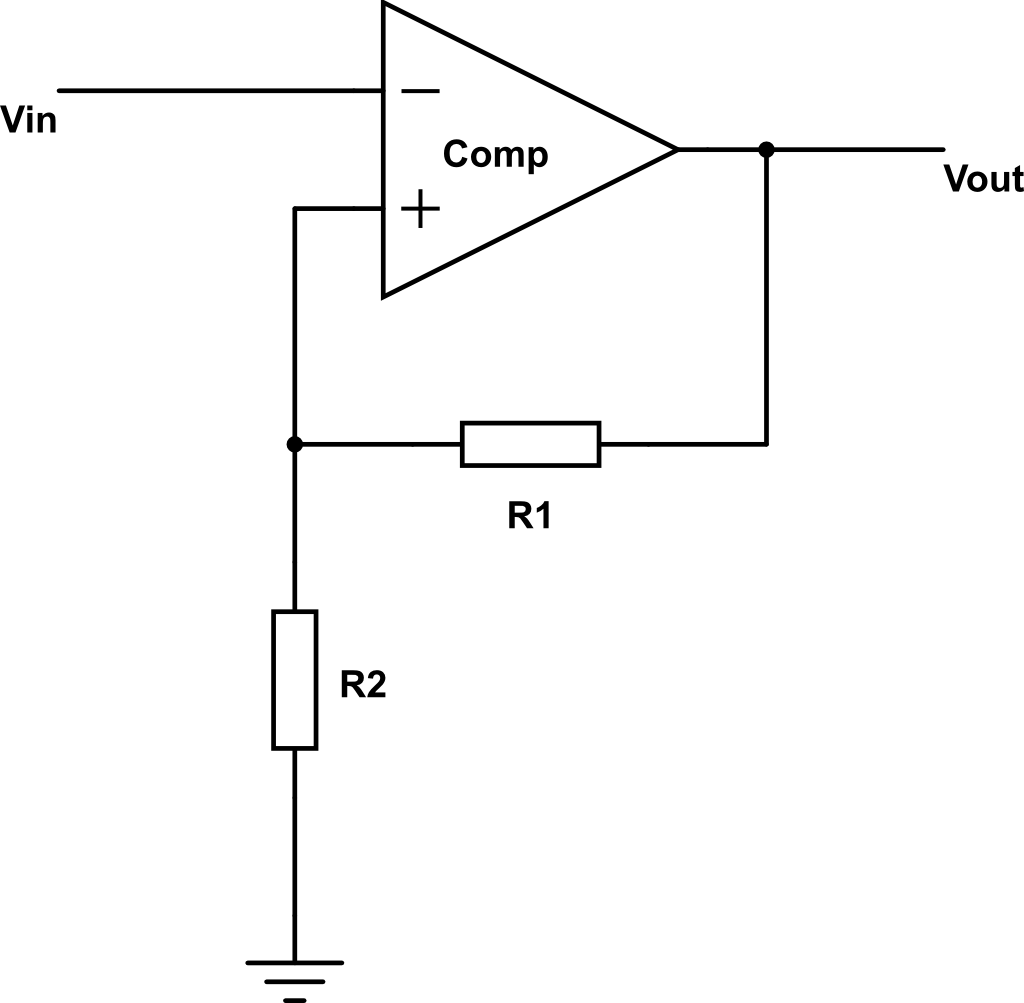
\includegraphics[width=\textwidth]{comparator.png}
		\caption{Schematische weergave van een comparator met hysterese op basis van een op-amp}
		\label{fig:comp-schem}
	\end{subfigure}
	\caption{De comparator}
	\label{fig:comp}
\end{figure}

Een simpele comparator is te maken door een op-amp te gebruiken zonder terugkoppelnetwerk. Omdat het ingangssignaal door de op-amp een groot aantal keer wordt versterkt naar een spanningsniveau wat de op de op-amp aangesloten energiebron niet kan leveren, zal het uitgangssignaal altijd gelijk zijn aan ofwel de negatieve voedingsspanning, ofwel de positieve, afhankelijk van het teken van de ingangs- en voedingsspanningen. We willen echter dat de uitgangsspanning pas ``clampt'' aan één van beide voedingsspanningen op het moment dat de ingangsspanning een bepaald spanningsniveau, de \textit{threshhold}-spanning ($V_{th}$) passeert. Dit noemt men hysterese. Hiertoe hebben we twee thresholds nodig: één voor een stijgend signaal ($V_{th,H}$) en één voor een dalend signaal ($V_{th,L}$). Dit is gevisualiseerd in figuur \ref{fig:comp-werk}. We bereiken deze hysterese door een gedeelte van de uitgangsstroom via een spanningsdeling terug te voeren naar de positieve ingang. Dit levert het circuit zoals gegeven in figuur \ref{fig:comp-schem} op, waarbij de bijbehorende threshholds dan zijn te berekenen aan de hand van de volgende vergelijkingen:

\begin{subequations}
	\begin{equation}
		V_{th,H} = \frac{R_{1}}{R_{1}+R_{2}}V_{max}
		\label{eq:comp-H}
	\end{equation}

	\begin{equation}
		V_{th,L} = \frac{R_{1}}{R_{1}+R_{2}}V_{min}
		\label{eq:comp-L}
	\end{equation}
	\label{eq:comp}
\end{subequations}

\noindent
Hierin zijn $V_{max}$ en $V_{min}$ respectievelijk de positieve en negatieve voedingsspanning op de op-amp.

Het uitgangssignaal van de comparator wordt hiermee dus een blokgolf met een frequentie die afhankelijk is van de ingangsspanning op de integrator. Deze uitgangsspanning wordt voor het oscillatie-effect nu via een inverterende versterker teruggevoerd aan de integrator en daarmee is de lus gesloten en de relaxatie-oscillator voltooid.

\subsection{Inverterende versterker}
Omdat de comparator en de integrator beide opgesteld zijn in de inverterende configuratie, zal het uiteindelijke signaal wat dus ook dient als ingangssignaal eerst nog een keer geïnverteerd moeten worden. Daarnaast kunnen we hiermee het spanningsniveau aan de ingang van de integrator nog wat aanpassen. 

\begin{wrapfigure}{r}{0.5\textwidth}
	\centering
	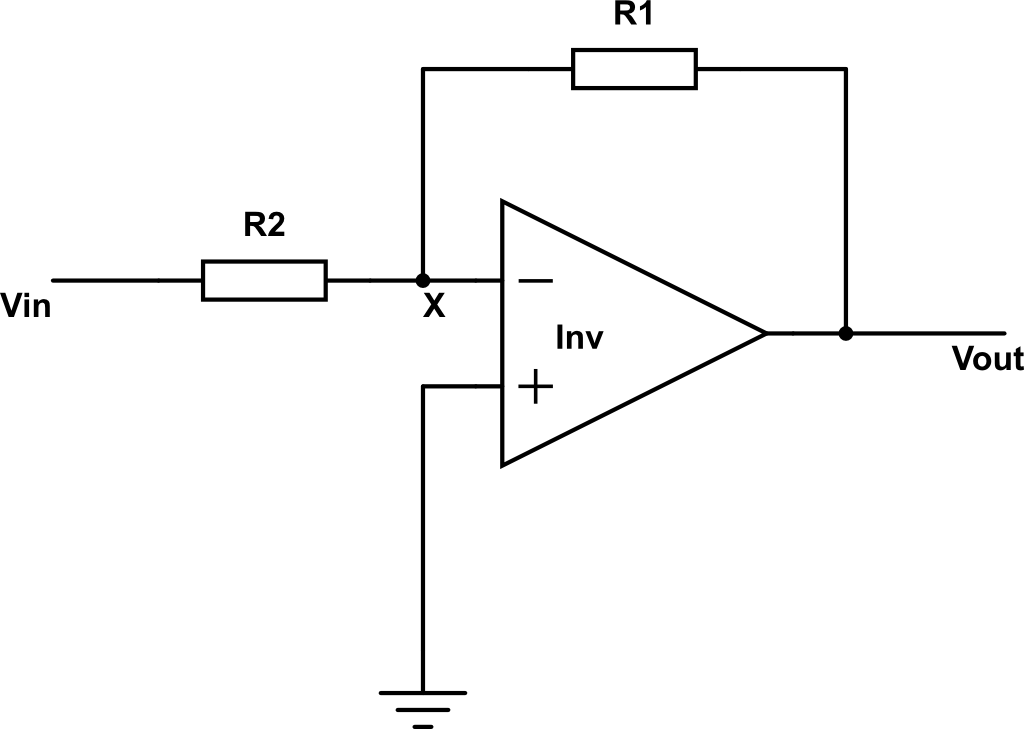
\includegraphics[width=0.4\textwidth]{inverterende-versterker.png}
	\caption{Schematische weergave van de inverterende versterker op basis van een op-amp}
	\label{fig:inv-ver}
\end{wrapfigure}

We doen dit met een normale op-amp in de inverterende configuratie (figuur \ref{fig:inv-ver}), met een combinatie van weerstanden die het ingangssignaal verzwakt ($R_{2}>R_{1}$). Om de uitgangsspanning als functie van de ingangsspanning te berekenen gebruiken we weer een knooppuntsvergelijking in knooppunt X:

$$\frac{V_{x}-V_{in}}{R_{2}} +\frac{V_{x}-V_{out}}{R_{1}} = 0$$

\noindent
Gebruikmakend van de nulconditie voor op-amps levert dit:

$$-\frac{V_{in}}{R_{2}} - \frac{V_{out}}{R_{1}} = 0$$

\noindent
En dus is de uiteindelijke overdracht:

\begin{equation}
	V_{out} = -\frac{R_{1}}{R_{2}}V_{in}
	\label{eq:inv-ver}
\end{equation}

\noindent
En hiermee is de relaxatie-oscillator compleet. 

\section{Afleiding}

We kunnen de voorgaande individuele overdrachten samenvoegen tot één vergelijking om de tijd te berekenen die de integrator er over doet om de spanning één keer van hoog naar laag (of andersom) te laten gaan, dit is dus een halve periode. Hiervoor nemen we de vergelijking voor de integrator (\ref{eq:int}) er nogmaals bij:

$$V_{out,int} = -\frac{V_{in,int}}{R_{pot}C} t - V_{0}$$

\noindent
Hierin zijn $R$, $C$, $V_{out,int}$ en $V_{0}$ bekend en wordt $V_{in,int}$ gegeven door de uitgangsspanning van de inverterende versterker:

$$V_{out,int} = -\frac{-\frac{R_{a}}{R_{b}}V_{in,inv}}{R_{pot}C} t - V_{0}$$

\noindent
$V_{in,inv}$ wordt op zijn beurt gegeven door ofwel $V_{max}$ ofwel $V_{min}$ uit de comparator:

$$V_{out,int} = -\frac{-\frac{R_{a}}{R_{b}}V_{max,comp}}{R_{pot}C} t - V_{0}$$
$$V_{out,int} = -\frac{-\frac{R_{a}}{R_{b}}V_{min,comp}}{R_{pot}C} t - V_{0}$$

\noindent
Als we echter kijken naar het diagram in figuur \ref{fig:comp-werk} zien we dat $V_{out,int}$, $V_{max,comp}$ en $V_{0}$ op toppen van de zaagtand aan elkaar gelijk zijn en $V_{out,int}$, $V_{min,comp}$ en $V_{0}$ in dalen aan elkaar gelijk zijn en dus kunnen we deze uitdelen:

$$1 = -\frac{-\frac{R_{a}}{R_{b}}}{R_{pot}C} t - 1$$
$$-1 = -\frac{\frac{R_{a}}{R_{b}}V_{min,comp}}{R_{pot}C} t + 1$$

\noindent
Dit levert na oplossen voor $t$ in beide gevallen op:

\begin{equation}
	t = 2\frac{R_{b}R_{pot}C}{R_{a}}
\end{equation}
\noindent
Waarbij geldt dat $T=2t$ en $f=\frac{1}{T}$
\begin{equation}
\label{eq:freqOscillator}
	f(R_{pot}) = \frac{R_a}{4 \cdot R_{b}R_{pot}C}
\end{equation}

\end{document}